\documentclass[]{article}
\usepackage{graphicx}

%opening
\title{Carbon elastics for HMS commissioning at 1 pass}

\begin{document}

\maketitle


\section{Introduction}

The first excited state of carbon elastics will be used to test the HMS optics.
Important to following the HMS cycling procedure.
The running conditions are given in table~\ref{tab:kin}.
Rates are listed is the table~\ref{tab:rates} assuming a 1uA beam current.
The inelastic evenst are plotted for various kinematic quantities in Fig.~\ref{fig:kin}
and for different combinations of focal plane quantities in Fig.~\ref{fig:inelastic}.
The elasitc 4.4~MeV events are plotted for different combinations
 of focal plane quantities in Fig.~\ref{fig:elastic44}. The elastic events are in a narrow part of the 
 of xfp and Fig.~\ref{fig:xfp} shows a comparison of the inelastic and elastic events rates.
 the elastic events dominate.

\begin{table}[h]
	\begin{center}
		\begin{tabular}[]{|c|c|} \hline\hline
			beam energy: & 2218 MeV\\ \hline
			HMS momentum & -2201.54 MeV \\ \hline
			HMS angle & 13.5 deg \\ \hline
			HMS collimator & Sieve \\ \hline
			beam current: & 3 $\mu$A\\ \hline
			fast raster: & off\\ \hline
			target: & 0.5\% carbon\\ \hline
		\end{tabular}
		\caption{Kinematics}
		\label{tab:kin}
	\end{center}
\end{table}
\begin{table}[h]
	\begin{center}
		\begin{tabular}[]{|c|c|} \hline\hline
			Inelastic & 370 Hz\\ \hline
			4.4 elastic state &  750 Hz\\ \hline
			ground state & 1 Hz \\ \hline
		\end{tabular}
		\caption{Rates assuming 1uA beam current}
\label{tab:rates}
	\end{center}
\end{table}

\begin{figure}	
	\begin{center}
		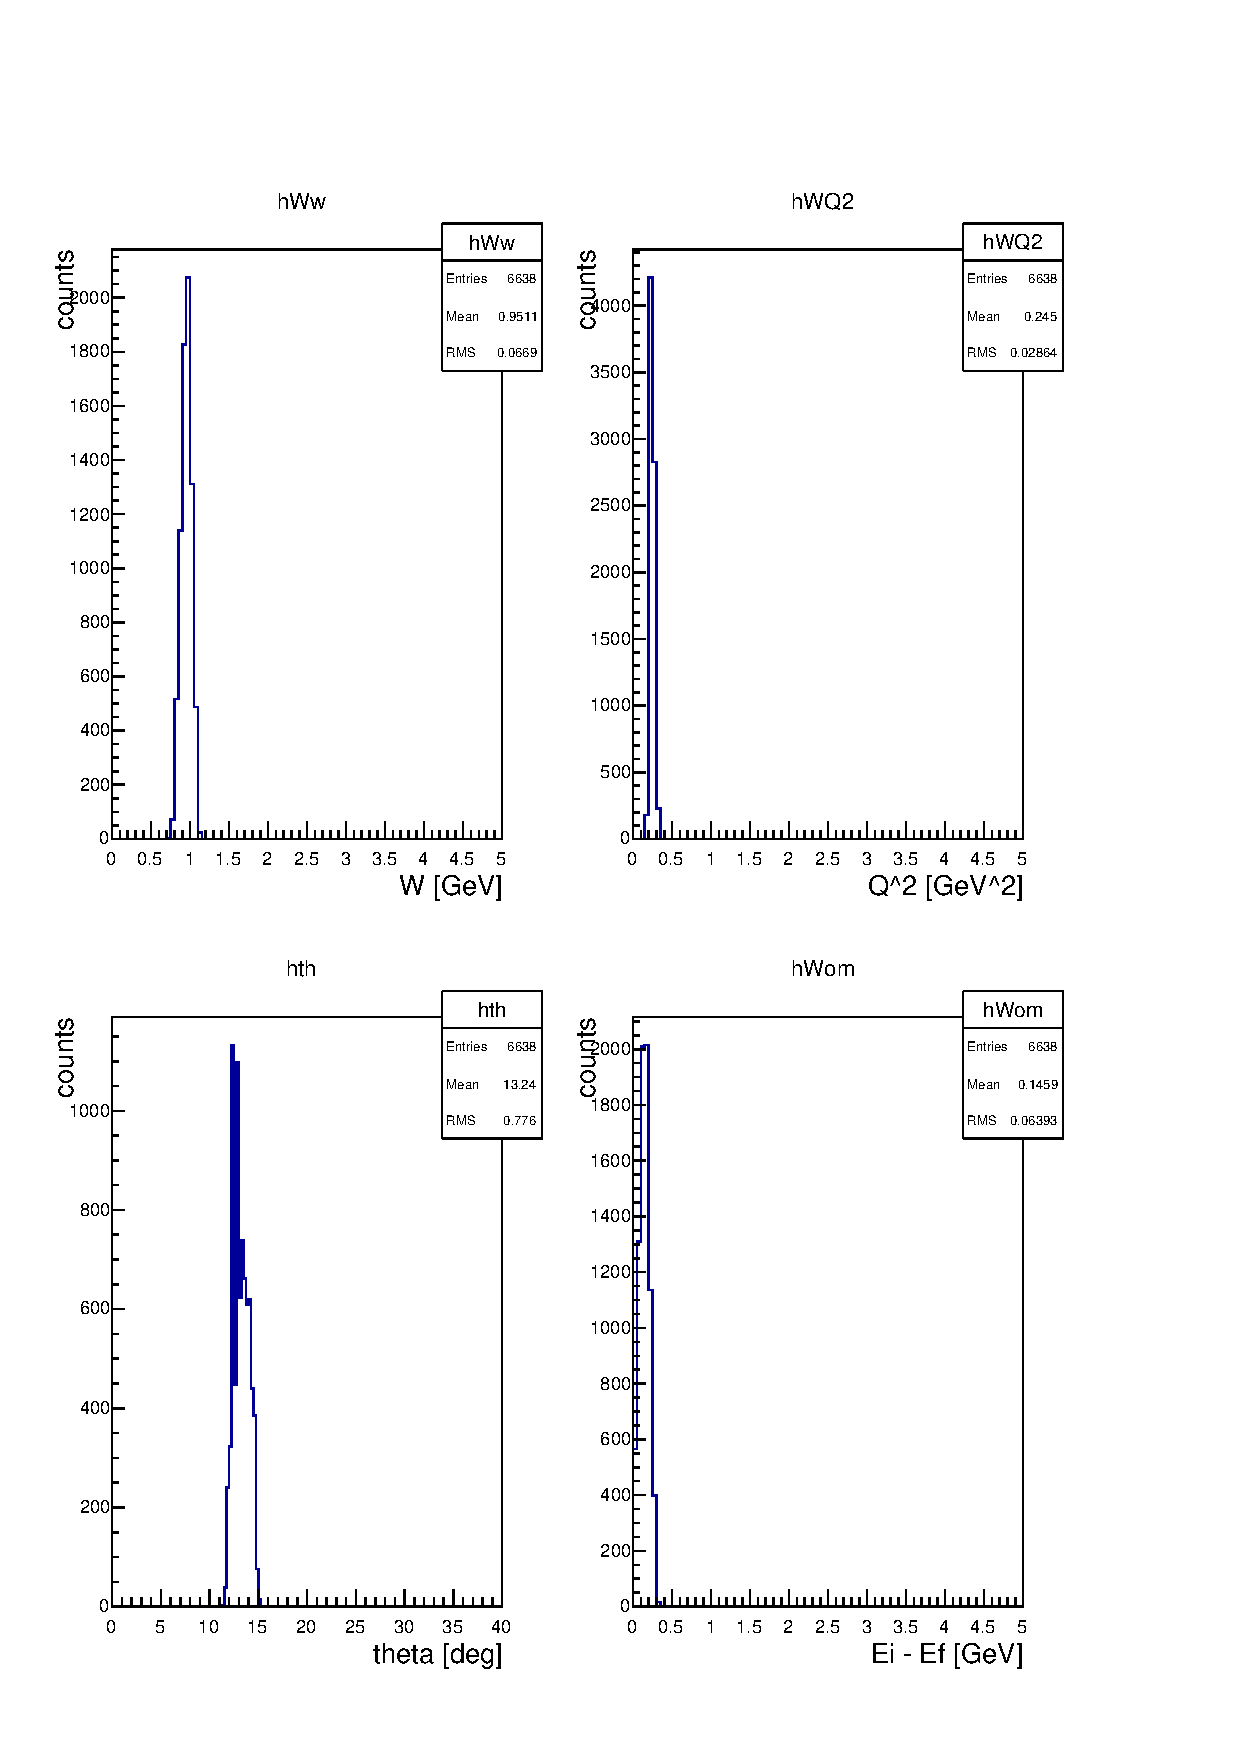
\includegraphics[width=0.98\columnwidth]{hms_pointtarg_13p5deg_2gev_wc_mscat_vac_sieve_car44_kin.pdf}
	\end{center}
	\caption{Plots of Inelastic events versus kinematic quantities. Y-axis is rate for 20uA. }
	\label{fig:kin}
\end{figure}


\begin{figure}	
\begin{center}
	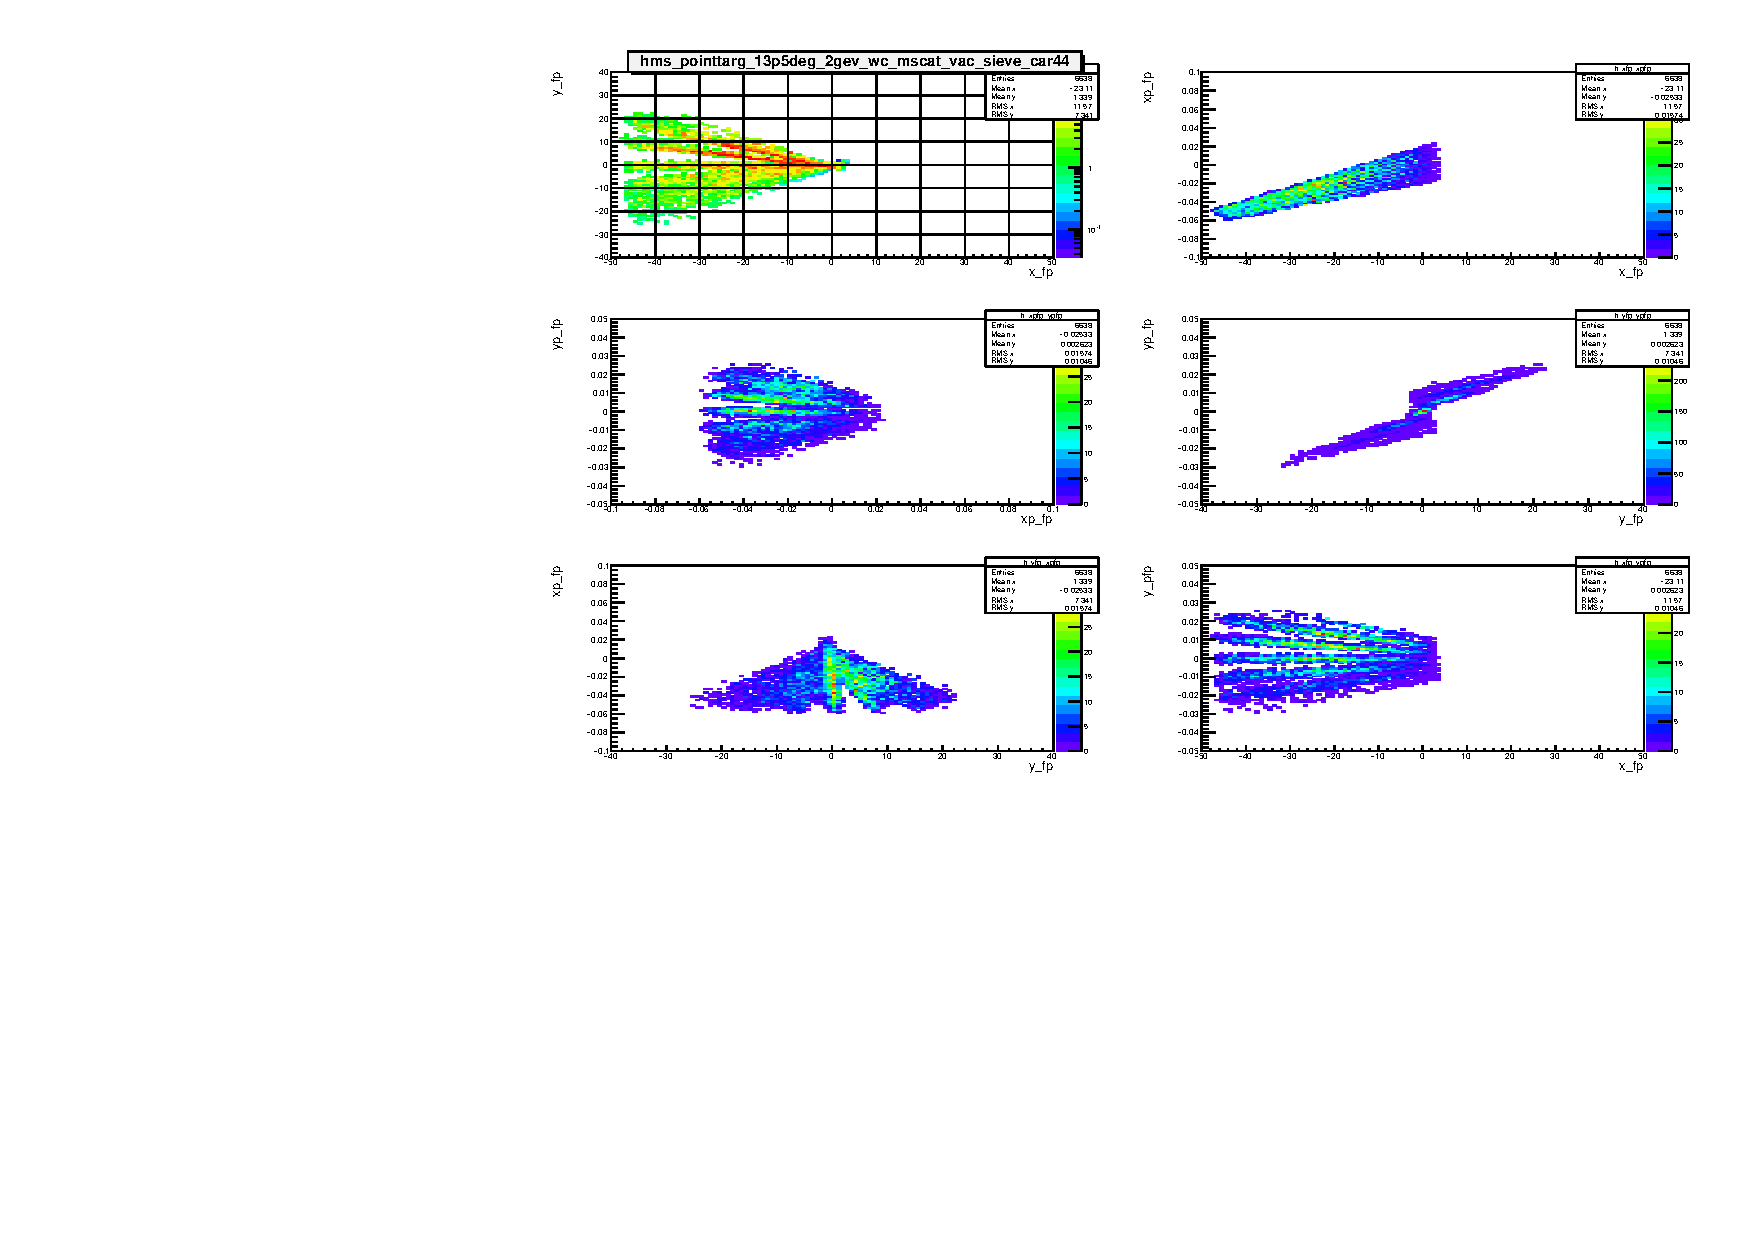
\includegraphics[angle=90]{hms_pointtarg_13p5deg_2gev_wc_mscat_vac_sieve_car44_inelastic.pdf}
\end{center}
\caption{Inelastic events in focal plane for different combinations of quantities. Xfp and Yfp
	are in cm.}
\label{fig:inelastic}
\end{figure}

\begin{figure}	
	\begin{center}
		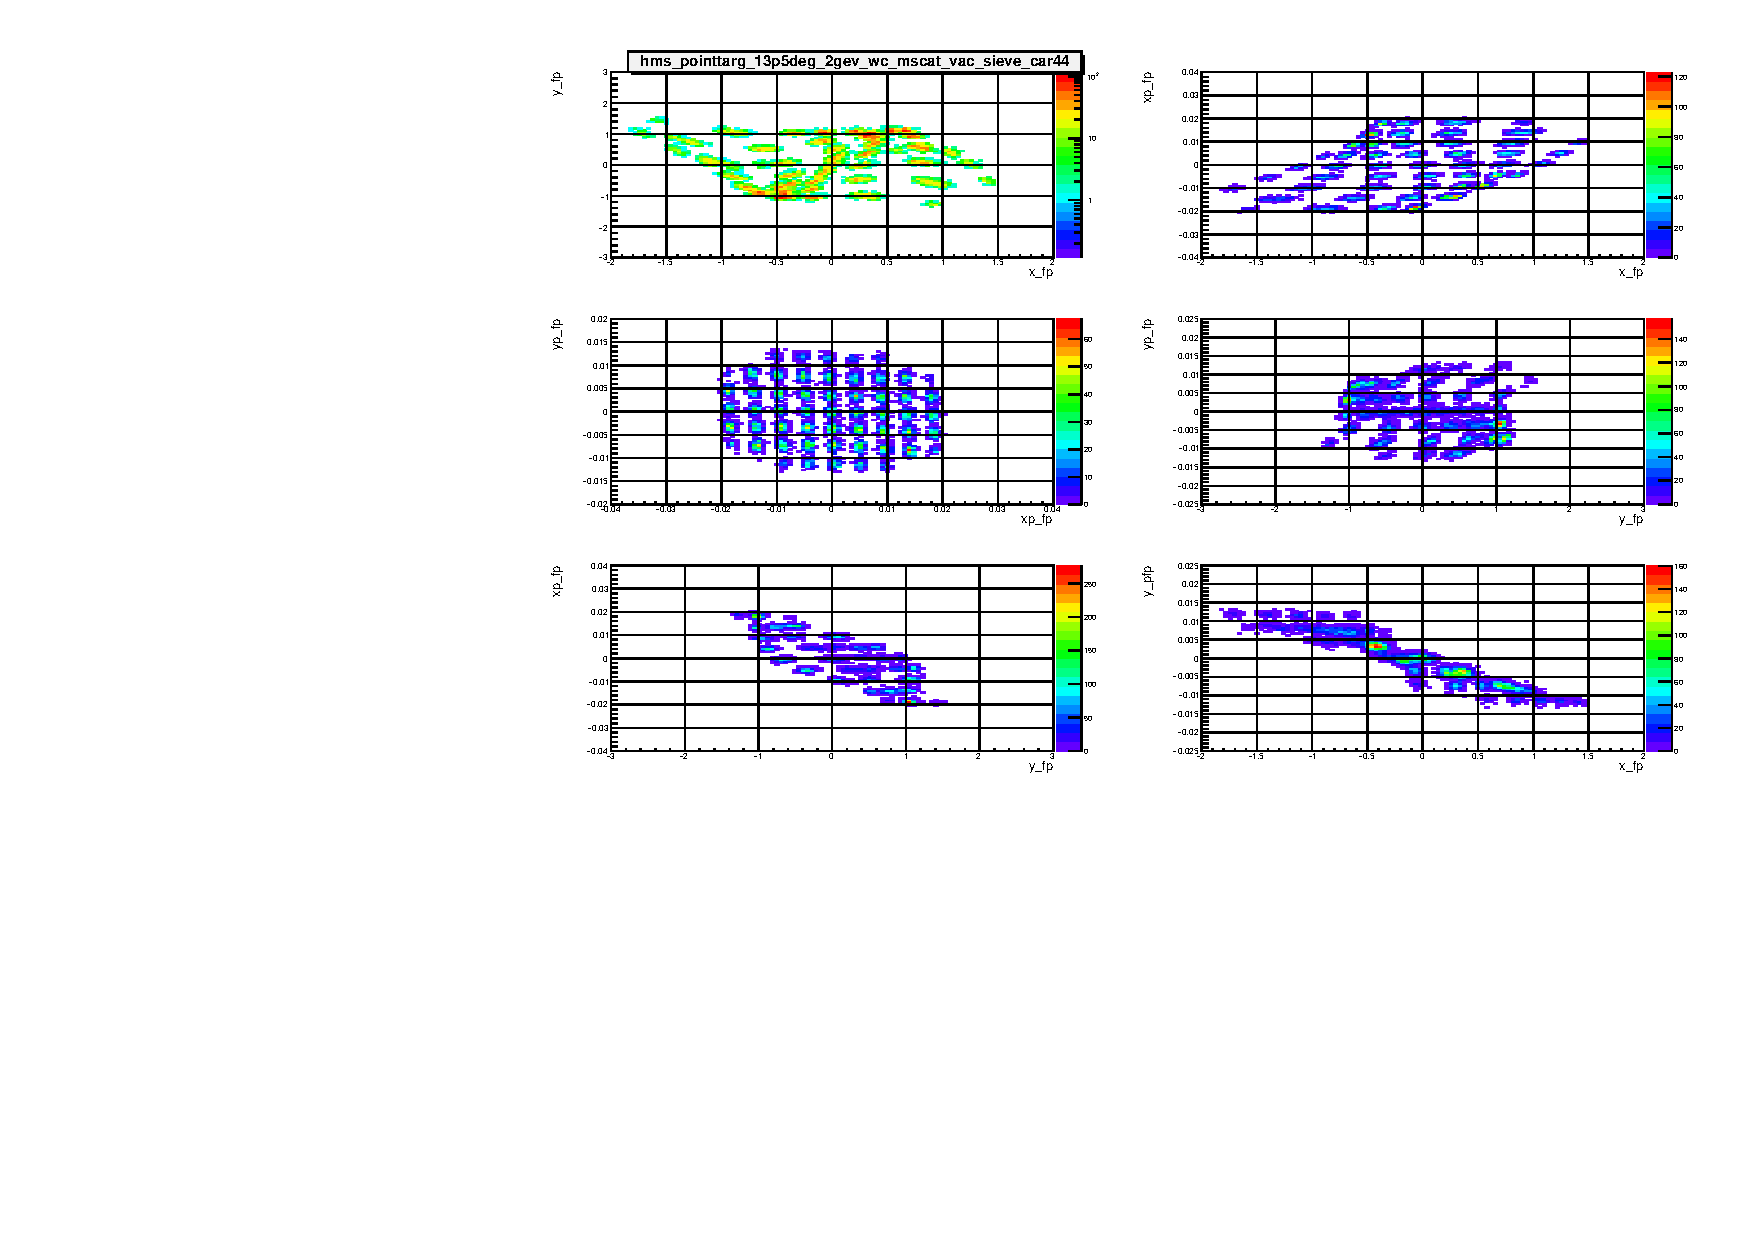
\includegraphics[angle=90]{hms_pointtarg_13p5deg_2gev_wc_mscat_vac_sieve_car44_44.pdf}
	\end{center}
	\caption{Elastic carbon 4.4 state events in focal plane for different combinations of quantities. Xfp and Yfp
	are in cm.}
	\label{fig:elastic44}
\end{figure}

\begin{figure}	
	\begin{center}
		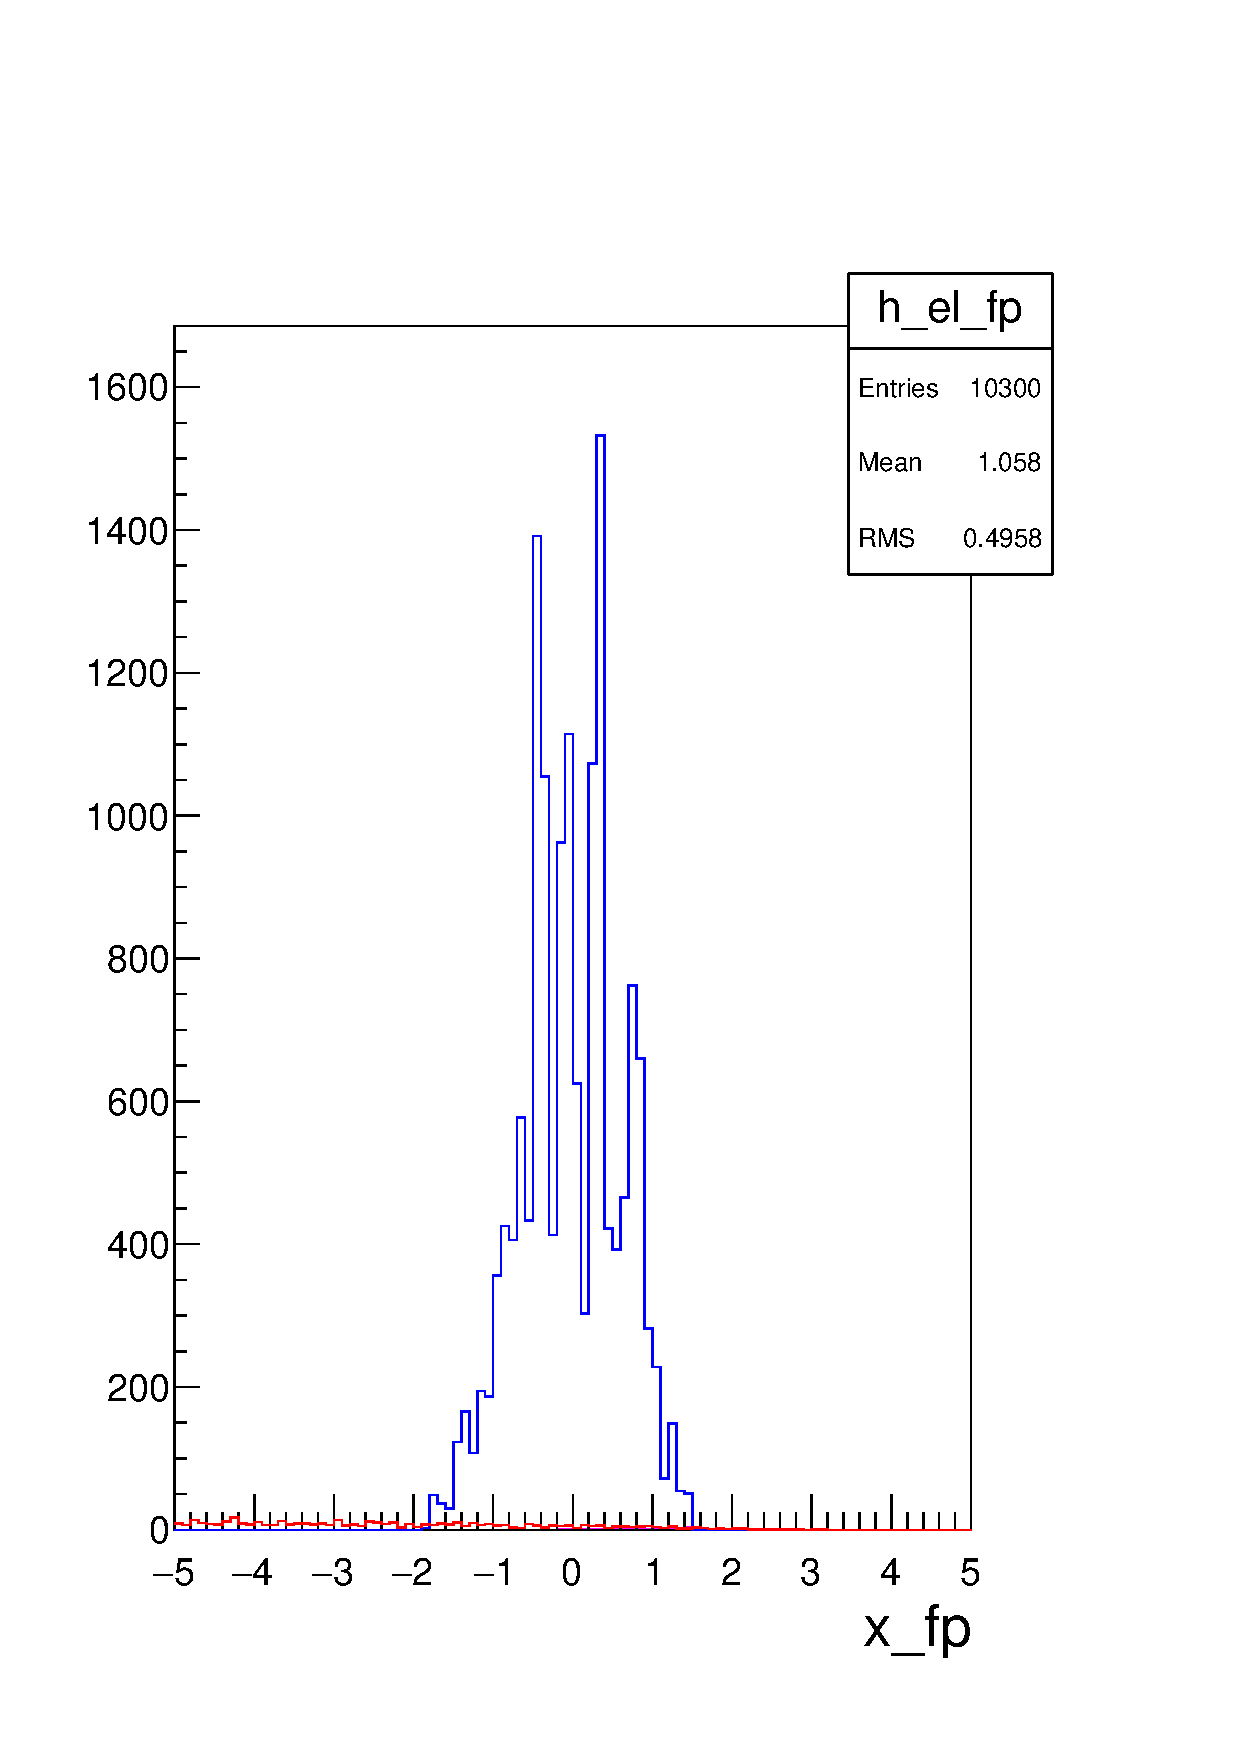
\includegraphics[width=0.98\columnwidth]{hms_pointtarg_13p5deg_2gev_wc_mscat_vac_sieve_car44_xfp.pdf}
	\end{center}
	\caption{Comparison between distribution of inelastic events (red) and elastic 4.4~MeV events (black)
		 in narrow part of xfp. Y-axis is rate for 20uA.  }
	\label{fig:xfp}
\end{figure}


\section{Surveys}

The surveys for the HMS are given in the Table.  Pointing is given in the spectrometer 
coordinate system with +X downwards and +Y towards smaller angles.
	\begin{table}[h]
		\begin{center}
			\begin{tabular}[]{|c|c||c|c|} \hline\hline
				Survey & Angle  & Horizontal point (Y$_{spec}$) & Vertical point (X$_{spec}$)\\ \hline
				C1792R & 40.534 & +3.45& +0.91\\ \hline
				C1807R & 40.013 & +3.29 & +0.94 \\ \hline
				C1809R & 50.00  & +2.92 & +1.07 \\ \hline
			\end{tabular}
			\caption{Surveys of the HMS}
		\end{center}
	\end{table}
	
	\section{First order optics}
	HMS first order forward optics:
\begin{eqnarray}
	xfp (mm) &=& -3.41*xtar (mm) - 0.02*xptar (mr) +37.0*delta \\
	xpfp (mr) &=& -.04*xtar (mm) - .29*xptar (mr) - 0.4*delta \\
	yfp (mm) &=& -2.2*ytar (mr) - 0.02*yptar (mr)  \\
	ypfp (mr) &=& -2.62*ytar (mm) - 0.42*yptar (mr) 
\end{eqnarray}
	
	HMS first order reconstruction optics.
\begin{eqnarray}
	xptar (mr) = 0.34 xfp ( mm) - 3.15 xpfp (mr) \\
	delta   = 0.026 xfp  (mm)  - 0.009 xpfp (mr) \\
	ytar  (mm) = -.38 yfp (mm) - 0.086ypfp (mr) \\
	yptar  (mr)= 0.26 yfp (mm) - 2.1 ypfp (mr) 
\end{eqnarray}

\end{document}
